
\section{Quantum Pirate Game}
\label{sec:quantum_pirate}

The original Pirate Game is posed from the point of view of the captain. How should she allocate the treasure to the crew in order to maximize her payoff?
We can find the a pure strategy Nash equilibrium in the original Pirates Game and, while the solution may seem unexpected at first sight, it is fully described using backwards induction. 

When modelling this problem from a quantum theory perspective we are faced with some questions, such as:

\begin{itemize}
\item Will the initial conditions provide different equilibria? 

\item What are the similarities with the classical problem? 

\item Will the quantum version of the problem be equally strictly determined?

\item Is it possible for a captain, in a situation where we have more than two pirates left, to acquire all the coins?

\end{itemize} 

The main difference from the original problem will rely on how the system is set up and the fact that we will allow quantum strategies. 
We propose to study this problem for a $3$ player game and trying to extrapolate for $N$ players. 

We will analyse the role of entanglement and superposition in the game system. 

Another aspect worth studying is the variation in the coin distribution on the payoff functions for the players. We are particularly interested in studying the classical equilibrium where the captain retains $99$ coins and gives a single coin to the player with the lowest rank. Moreover we want to study what happens when the captain tries to get all the coins.



\subsection{Quantum Model}
\label{subsec:description_2}

In order to model the problem we will start by defining it using the definition of quantum game ($\Gamma$), referred in \ref{eq:quantum_game_six_tuple}, Section \ref{sec:background_quantum_game_theory}\cite{Fra2011a}.

We want to keep the problem as close to the original as possible in order to better compare the results. Thus we will analyse the game from the point of view of the captain. Will her best response change?

For the purpose of demonstration this problem could be described using $3$ players; the lowest number of players that has an equilibrium in which the captain has to bribe another pirate. 

We begin by assigning an offset to each pirate (in order to identify her), as in the Section \ref{subsec:description}. The captain is number $1$ and the lower the number the higher the rank. 



\subsubsection{Game system: Setting up the Initial State}
\label{subsec:pirates_initialstate}

A game $\Gamma$ can be viewed as a system composed by qubits manipulated by players. We will use the definition of quantum game discussed in Section \ref{sec:background_quantum_game_theory} ($\Gamma=(\mathcal{H}^{2^{a}},\: N,\:\vert\psi_{in}\rangle,\:\xi,\:\{\mathcal{U}_{j}\},\:\{E_{i}\})
$), to model our game system. Akin to the Quantum Ultimatum game desbribed in \cite{Fra2011}, our objective is to apply that quantization scheme to the normal form representation of the game tree in Figure \ref{fig:pg_architecturegametree:extensiveform}.


In this $3$ player game there will be $5$ qubits representing the actions or the players decision; three qubits will represent the first voting round, the other two will portray the actions of the second voting round.
The number of qubits needed to represent the game grows exponentially with the number of players. For $N$ players we need $\sum_{i=2}^{N}{i}$ qubits. With 8 players, this game would already be impractical to simulate in a classical computer. In this regard a quantum computer may enhance our power to simulate this kinds of experiments \cite{Rieffel2011}.

The mapping function $\xi$ that assigns each action/qubit $\varphi_{j}$ ( with $j=\{ 1, 2, 3, 4, 5\}$), to a player is represented on Equation \ref{playerxiximapping}. 

\begin{equation}
\xi(j)=\begin{cases}
1 & ,\; if\; j=1;\\
2 & ,\; if\; j\in\{2,4\};\\
3 & ,\; if\; j\in\{3,5\}.
\end{cases}
\label{playerxiximapping}
\end{equation}


With $3$ players and $5$ actions our system with be represented in a $\mathcal{H}^{32}$ using a state $\psi$. This means that to represent our system we will need $2^{5}\times 1$ vectors, our system grows exponentially with the number of players/qubits. Each pure basis  of $\mathcal{H}^{32}$, shown in Equation \ref{putadevida}, will represent a possible outcome in the game. We assign a pure basis as $\vert 0\rangle = \vert C\rangle$ (``C'' from ``Cooperate''), and $\vert 1\rangle = \vert D\rangle$ (``D'' from ``Defect''). 


\begin{equation}
\begin{split}
\mathcal{B}= \{ \vert 00000\rangle , \vert 00001\rangle , \vert 00010\rangle , \vert 00011\rangle , \vert 00100\rangle , \vert 00101\rangle , \vert 00110\rangle , \vert 00111\rangle, \\
 \vert 01000\rangle , \vert 01001\rangle , \vert 01010\rangle , \vert 01011\rangle , \vert 01100\rangle , \vert 01101\rangle , \vert 01110\rangle , \vert 01111\rangle, \\
 \vert 10000\rangle , \vert 10001\rangle , \vert 10010\rangle , \vert 10011\rangle , \vert 10100\rangle , \vert 10101\rangle , \vert 10110\rangle , \vert 10111\rangle, \\
 \vert 11000\rangle , \vert 11001\rangle , \vert 11010\rangle , \vert 11011\rangle , \vert 11100\rangle , \vert 11101\rangle , \vert 11110\rangle , \vert 11111\rangle \}
\end{split}
\label{putadevida}
\end{equation}



%\begin{figure}[h]
%\centering 
%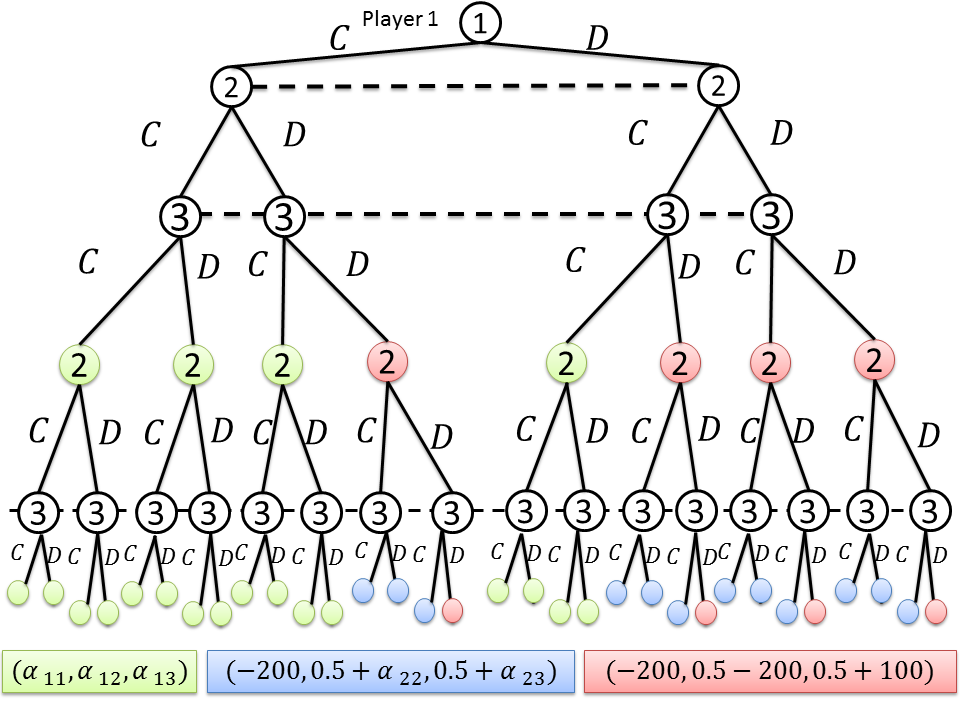
\includegraphics[scale=0.55]{Figures/architecture/GameTree/Slide1.png}
%\caption{Game tree representation for a $3$-player game. Red circles represent failed proposals, green represent accepted proposals. }
%\label{fig:pg_architecturegametree}
%\end{figure}


\begin{comment}
\begin{center}
\begin{tabular}{c|cccc|cccc}
\hline 
\multicolumn{5}{c}{$\tau_{1}=\mathcal{C}_{1}$} & \multicolumn{4}{c}{}\tabularnewline
\hline 
\multicolumn{1}{c}{} & Player 3: CC & Player 3: CD & Player 3: DC & Player 3: DD & Player 3: CC & Player &  & \tabularnewline
\cline{2-9} 
Player 2: CC & (1,1,0) & (0,2) &  &  &  &  &  & \tabularnewline
Player 2: CD & (2,0) & (0,0) &  &  &  &  &  & \tabularnewline
Player 2: DC &  &  &  &  &  &  &  & \tabularnewline
Player 2: DD &  &  &  &  &  &  &  & \tabularnewline
\hline 
\end{tabular}
\par\end{center}
\end{comment}


The initial system ($\vert \psi_{0}(\gamma) \rangle$), will be set up by defining an entanglement coefficient $\gamma$, that affect the way the five qubits (belonging to the three pirate players), are related; this is shown in Equation \ref{eq:estado_inicial_pg}. 
We will entangle our state by applying the gate $\mathcal{J}$ \cite{Letters2002}. The parameter $\gamma$ becomes a way to measure the entanglement in the system\cite{Eisert2008}. 

The concept of entanglement is crucial to explain some phenomena in Quantum Mechanics (Section \ref{subsec:entanglement}).We analysed the role of the entanglement of the system since other examples researched pointed to it being the prominent factor regarding behaviour changes from the classsical perspective\cite{Fra2011a}\cite{Fra2011}\cite{Letters2002}\cite{Khan2011}\cite{Ricketts2006}. 

We can interpret the existence (or non-existence), of entanglement or superposition in the initial system as an unbreakable contract between the players\cite{Piotrowski}. The initial state starts by revealing a group of pirates that cooperate by default. We chose this initial set-up because it is prevalent in the literature\cite{Eisert2008}\cite{Fra2011a}\cite{Fra2011}\cite{Letters2002}, and we want to test if there is any equilibrium situation where the first captain can pass her proposal while taking all the 100 coins. 


%The index $0$ represents the depth of the game tree which can be examined in Figure \ref{fig:pg_architecturegametree}.

Due to the nature of quantum mechanics we have to pay attention of how we set-up our architecture; we cannot copy or clone unknown quantum states (No-cloning Theorem)\cite{Rieffel2011}. 



\begin{equation}
\mathcal{J}=exp\left\{ i\frac{\gamma}{2}\left[\begin{array}{cc}
0 & 1\\
1 & 0
\end{array}\right]\otimes\left[\begin{array}{cc}
0 & 1\\
1 & 0
\end{array}\right]\otimes\left[\begin{array}{cc}
0 & 1\\
1 & 0
\end{array}\right]\otimes\left[\begin{array}{cc}
0 & 1\\
1 & 0
\end{array}\right]
\otimes\left[\begin{array}{cc}
0 & 1\\
1 & 0
\end{array}\right]
\right\}
\label{eq:matrix_exponencial_esoterica}
\end{equation} 

\begin{center}
\begin{equation}
%\vert \psi_{0}(\gamma) \rangle= cos( \frac{\gamma}{2})\vert 00\rangle+ isin(\frac{\gamma}{2})\vert 11 \rangle, \gamma \in (0,\pi)
\begin{split}
\vert\psi_{ini}(\gamma)\rangle=exp\left\{ i\frac{\gamma}{2}\left[\begin{array}{cc}
0 & 1\\
1 & 0
\end{array}\right]\otimes\left[\begin{array}{cc}
0 & 1\\
1 & 0
\end{array}\right]\otimes\left[\begin{array}{cc}
0 & 1\\
1 & 0
\end{array}\right]\otimes\left[\begin{array}{cc}
0 & 1\\
1 & 0
\end{array}\right]\otimes\left[\begin{array}{cc}
0 & 1\\
1 & 0
\end{array}\right]\right\} \vert00000\rangle \\
=cos(\frac{\gamma}{2})\vert00000\rangle+isin(\frac{\gamma}{2})\vert11111\rangle,\gamma\in(0,\frac{\pi}{2})
\end{split}
\label{eq:estado_inicial_pg}
\end{equation}
\end{center}



\subsubsection{Strategic Space}
\label{subsec:strategic_space}

In Equation \ref{eq:quantum_game_six_tuple} ($\Gamma=(\mathcal{H}^{2^{a}},\: N,\:\vert\psi_{in}\rangle,\:\xi,\:\{\mathcal{U}_{j}\},\:\{E_{i}\})
$), there is the notion of a subset of unitary operators that the players can use to manipulate their assigned qubits.

Each player will be able to manipulate at least one qubit in the system. Those qubits (of the form \ref{eq:opvarphiquantumstates}) are $\vert\varphi_{1}\rangle,\:\vert\varphi_{2}\rangle$, $\vert\varphi_{3}\rangle$, $\vert\varphi_{4}\rangle$, and $\vert\varphi_{5}\rangle$. The Equation \ref{putadevida} assigns the qubit $\vert\varphi_{1}\rangle$ to player $1$, qubits $\vert\varphi_{2}\rangle$ and $\vert\varphi_{4}\rangle$ to player $2$, the remaining qubits are assigned to player $3$. 

\begin{equation}
\varphi_{j} = a . \vert C \rangle + b . \vert D \rangle , j \in \{ 1, 2, 3, 4, 5 \}, \{ a,b \} \in \mathbb{C} : a^2 + b^2 =1
\label{eq:opvarphiquantumstates}
\end{equation}

Each player will be able to manipulate her assigned qubits $j$ with an unitary operator of the form shown in Equation \ref{eq:general_unitary_special_one} (shown in Section \ref{sec:background_quantum_game_theory}). However in  order to explore the potential of quantum strategies, \cite{Eisert2008} proposes that it is sufficient to restrict the strategic space span by to the $2$-parameter (polar coordinates), set of matrices in Equation \ref{eq:operadoresinfinitus}, with $ \theta \in ( 0, \pi )$, and $\phi \in ( 0, \frac{\pi}{2})$. We will try to use the strategic space $\mathcal{U}_{j}(\theta,\phi)$ to represent our player's actions.



\begin{equation}
\mathcal{U}_{j}(\theta,\phi) = \left[\begin{array}{cc}
cos(\frac{\phi}{2}) & e^{i\phi}sin(\frac{\phi}{2})\\
-e^{-i\phi}sin(\frac{\phi}{2}) & cos(\frac{\phi}{2})
\end{array}\right] , j \in \{ 1, 2, 3, 4, 5 \}, \theta \in ( 0, \pi ) , \phi \in ( 0, \frac{\pi}{2})
\label{eq:operadoresinfinitus}
\end{equation}


 However the two operators that correspond to the original classical actions of voting ``Yes'' or to Cooperate, and voting ``No'' (Defect) are not entirely characterized by the subset $\mathcal{U}_{j}(\theta, \phi)$. These classical actions belong to a subset $S_{j}$ described in Equation \ref{eq:operators_piratas_quanticos}.  
The classical cooperation operator will be represented by the Identity operator ($o_{j0}$, where $j$ identifies the qubit that the respective player will act upon). When assigned to a qubit this operator will leave it unchanged. This operator is described by Equation \ref{eq:operadoresinfinitus} when $\mathcal{U}(0,0)$.

The defection operator ($D$), is represented by one of Pauli's Operators - the Bit-flip operator. This operator was chosen because it performs the classical operation NOT on a qubit. 
Within the restricted space $\mathcal{U}_{j}$, approximate alternative for the defect operator in the set $\mathcal{U}_{j}$ is $\mathcal{U}_{j}(\pi, 0)$; they are interchangeable when $\gamma = 0$. For $\gamma >0$ we will include the pure strategy $D$ represented by the Bit-flip operator into our restricted strategic scape $\mathcal{U}_{j}$.



%These operators are also permutation matrices, so our players are in fact permuting the state of their qubit as in the roulette quantum model (Section \ref{subsec:quantum_roulette}).

\begin{equation}
S_{j} = \begin{cases}
C_{j} = o_{j0}=\left[\begin{array}{cc}
1 & 0\\
0 & 1
\end{array}\right]\\
D_{j} = o_{j1}=\left[\begin{array}{cc}
0 & 1\\
1 & 0
\end{array}\right]
\end{cases} , j \in \{ 1, 2, 3, 4, 5 \}
\label{eq:operators_piratas_quanticos}
\end{equation}

Each player will have a strategy $\tau_{i}$  which assigns a
unitary operator $U_{j}$ to every qubit $j$ that is manipulated
by the player (\inputencoding{latin1}{$j$$\in\xi^{-1}(i)$}\inputencoding{latin9}). $\tau_{2}= \{D_{2},C_{4}\}$ represents the strategy where the player $2$ votes $D$ in the first stage and $C$ in the second stage.


In Quantization schemas of the Prisoner's Dilemma\cite{Letters2002}\cite{Eisert2008}, and Quantum Ultimatum Game\cite{Fra2011}, the strategic space, described in Equation \ref{eq:operadoresinfinitus}, was analysed allowed a infinity of mixed quantum strategies. In the Quantum Roulette Game\cite{Salimi2009} and \cite{Meyer1999} we have a demonstration that in a classical two-person zero-sum strategic game, if only one player is allowed to adopt a quantum strategy, she has a better chance of winning the game. 

The notation for the pure basis as $\vert C\rangle$ refers to a quantum state and should not be confused as a Cooperate operator $C$ that is a matrix (the identity matrix). A original player quantum state (the qubits of the form $\varphi_{j}$) is defined by Equation \ref{eq:opvarphiquantumstates}.





\subsubsection{Final State}
\label{subsec:pirates_finalstate}

We can play the Pirate Game by considering a succession of steps or voting rounds. In each step we have a simultaneous move(the players sellect their strategies at the same time), however, considering the potential rounds the game has, we have a sequential game. 

With three players, the first move will correspond to the player 1 (or the captain), if the proposal fails we will proceed to the second step in the game, where the remaining two players will vote on a new proposal made by player 2 (who will be the new captain). 

This final state is calculated by constructing a super-operator, by performing the tensor product of each player chosen strategy, from Equation \ref{eq:operadoresinfinitus} or \ref{eq:operators_piratas_quanticos}. The super-operator, containing each player's strategy, will then be applied to the initial state,as shown in Equation\ref{eq:piratas_final_move}.

\begin{equation}
\vert\psi_{fin}\rangle=\otimes_{i=1}^{3}\otimes_{j\in\xi^{-1}(i)}\mathcal{U}_{j}\vert\psi_{ini}(\gamma)\rangle
\label{eq:piratas_final_move}
\end{equation}

In the Figure \ref{fig:pg_architecture3players} we have a representation of the game.We start by building our initial state $k-1$, then the players  select their strategies, a super operator is constructed by performing a tensor product of the selected operators. 

In order to calculate the expected payoff functions we need to de-entangle the system, before measuring. The act of measuring, in quantum computing, gives an expected value that can be understood as the probability of the system collapsing into that state. 

We can de-entangle the our $\mathcal{H}^{32}$ system by applying $\mathcal{J}^{\dagger}$ (Equation \ref{eq:piratas_final_move}), this will produce a final state that we will be able to measure. If we do not apply the inverse transformation $\mathcal{J}^{\dagger}$ we are introducing errors in the system (when the entanglement parameter $\gamma$ is different than $0$), because we are introducing a correlation between the qubits in the system. In the Figure \ref{fig:pg_architecture3players} we have represented the way we entangle and de-entangle the system.


\begin{figure}[h]
\centering 
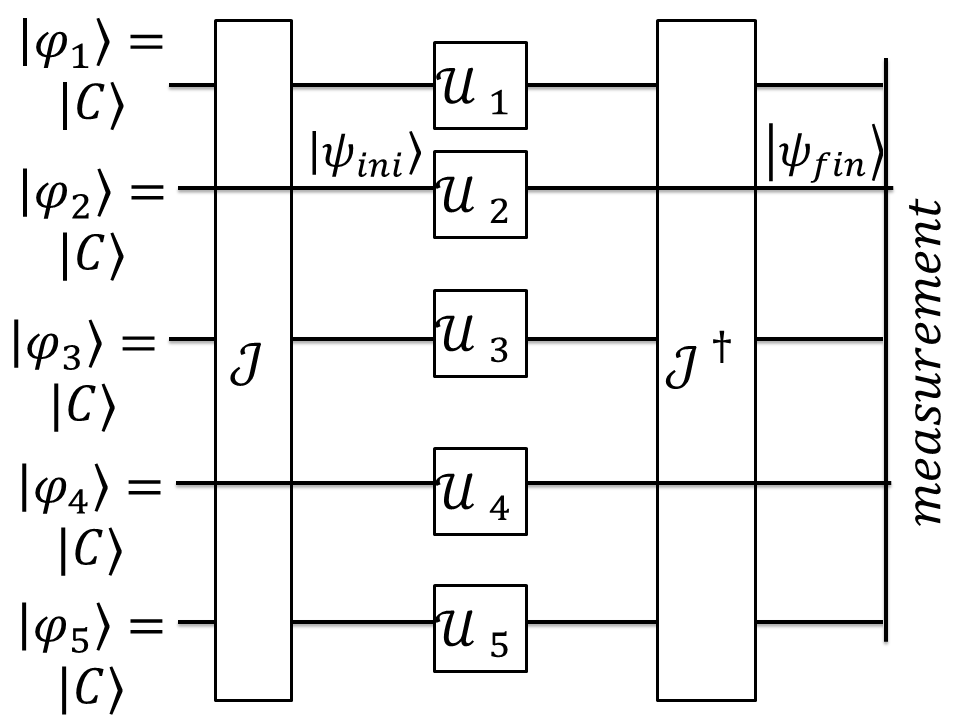
\includegraphics[scale=0.35]{Figures/architecture/esquema/esquema.png}
\caption{Scheme that represents the set-up of the $3$-player Pirate Game. Before we measure the final result we need to apply the transpose operator $\mathcal{J}^{\dagger}$. }
\label{fig:pg_architecture3players}
\end{figure}



\begin{comment}

In the original game the voting results are displayed between rounds, thus being an extensive form game. In the article ``Quantum information approach to the ultimatum game''\cite{Fra2011}, the authors model an extensive form game, and claim that it is more natural measuring the system between stages of the game (from a quantum perspective), instead of observing the actions taken by the players. However with our set-up measuring between rounds will destroy the initial entanglement which means that the effects of entanglement will only be present in the first stage of the game. 

This leads to the decision that to quantize the stages in the game we should be observing the actions taken by the players. The actions taken by the players will indicate whether the game stops (if the proposal is accepted), or if it ensues to a new stage (Figure \ref{fig:pg_architecture3players_architecture}). 

In order to preserve the consider the phenomenon of entanglement in the sub-games, while measuring the state after a stage (applying $J^{\dagger}$), methodology suggested by \cite{Fra2011} we would need to reapply an entanglement gate ($J_{2}^{\dagger}$), with a new entanglement parameter $\gamma_{2}$. This would introduce a new parameter introducing a new layer of complexity to the simulation; for each initial entanglement coefficient $\gamma$ we would have an infinity of entanglement coefficients for each sub-game. When the two entanglement coefficients are equal the probability distributions associated with each pure-base of the system the are equal to our approach of observing the actions taken by the players.


The next pirate in the hierarchy will then become the captain, and the previous captains will no longer be able to cast a vote (a symmetric Coin matrix will be used instead). 
Unlike the classic version, where the captain destined to be killed are tossed aside, in the quantum version they will be only thrown off board when we measure the final state and their expected utility is negative.
In this stage we must take into consideration that the players are pronouncing their votes taking into account their previous actions.
\end{comment}



\subsubsection{Utility}
\label{subsec:pirates_utility}

To build the expected payoff functionals for the three player situation we must take into account the sub-games created when the proposal is rejected. In Figure \ref{fig:pg_architecturegametree:extensiveform} we can see an extensive form representation of the game.

As defined on Equation \ref{eq:quantum_game_definition_payoff_func} ($ E_{i}=\sum_{b \in \mathcal{B}} u_{i}(b)\vert \langle b\vert \psi_{fin}\rangle\vert^{2}, u_{i}(b) \in \mathbb{R} $),for each player we must specify a utility functional that attributes a real number to the measurement of the projection of a basis in the quantum state that we get after the game. 


This measurement can be understood as a probability of the system collapsing into that state (that derives from the Born Rule, Section \ref{subsubsec:bornrule}).


These utility functions will represent the degree of satisfaction for each pirate after game by attributing a real number to a measurement performed to the system (as in Equation \ref{eq:quantum_game_definition_payoff_func}, Section \ref{sec:background_quantum_game_theory}). 
The real numbers used convey the logical relations of utility posed by the original problem description. Those numbers will represent the utility associated with the number of coins that a pirate gets $(\alpha_{ij})$, a death penalty $(-200)$, and a small incentive to climb the hierarchy $(0.5)$, and were derived from the classical analysis of the problem in Section \ref{subsubsec:analysis_PG3players}. 
As each pirate wants to maximize her utility, the Nash equilibrium will be thoroughly used to find the strategies that the pirates will adopt\cite{nash50}\cite{Nash51}.


We can observe in Figure \ref{fig:pg_architecturegametree:extensiveform} that in that we have three separate groups (denoted by the colour accents), of outcomes that share the same payoff, in the original problem. 
In our quantum scheme we can aggregate the pure-basis quantum states ($\mathcal{B}$), associates with a payoff in the following manner: 
\begin{itemize}
\item States where the first proposal is accepted - ``Accepted 1' (or $A_{1}$), with a green colour accent in Figure \ref{fig:pg_architecturegametree:extensiveform}:
\begin{itemize}
\item $\vert C,C,C,x_{4},x{5}\rangle$ or $\vert0,0,0,x_{4},x{5}\rangle$, with $x_{4} \in\{0,1\}$ and $x{5} \in \{0,1\}$;
\item $\vert D,C,C,x_{4},x{5}\rangle$ or $\vert1,0,0,x_{4},x{5}\rangle$, with $x_{4} \in\{0,1\}$ and $x{5} \in \{0,1\}$;
\item $\vert C,D,C,x_{4},x{5}\rangle$ or $\vert0,1,0,x_{4},x{5}\rangle$, with $x_{4} \in\{0,1\}$ and $x{5} \in \{0,1\}$;
\item $\vert C,C,D,x_{4},x{5}\rangle$ or $\vert0,0,1,x_{4},x{5}\rangle$, with $x_{4} \in\{0,1\}$ and $x{5} \in \{0,1\}$.
\end{itemize}
\item States where the first captain will be eliminated and the second player gets her proposal accepted  - ``Accepted 2'' (or $A_{2}$) with a blue colour accent in Figure \ref{fig:pg_architecturegametree:extensiveform}:
\begin{itemize}
\item $\vert D,D,D,C,x{5}\rangle$ or $\vert1,1,1,0,x{5}\rangle$, with $x{5} \in \{0,1\}$;
\item $\vert D,D,D,D,C\rangle$ or $\vert1,1,1,1,0\rangle$;
\item $\vert D,D,C,C,x{5}\rangle$ or $\vert1,1,0,0,x{5}\rangle$, with $x{5} \in \{0,1\}$;
\item $\vert D,D,C,D,C\rangle$ or $\vert1,1,0,1,0\rangle$;
\item $\vert C,D,D,C,x{5}\rangle$ or $\vert0,1,1,0,x{5}\rangle$, with $x{5} \in \{0,1\}$;
\item $\vert C,D,D,D,C\rangle$ or $\vert0,1,1,1,0\rangle$;
\item $\vert D,C,D,C,x{5}\rangle$ or $\vert1,0,1,0,x{5}\rangle$, with $x{5} \in \{0,1\}$;
\item $\vert D,C,D,D,C\rangle$ or $\vert1,0,1,1,0\rangle$.
\end{itemize}
\item States where all proposals are rejected  - ``Rejected 2' (or $R_{2}$)' with a red colour accent in Figure \ref{fig:pg_architecturegametree:extensiveform}:
\begin{itemize}
\item $\vert D,D,D,D,D\rangle$ or $\vert1,1,1,1,1\rangle$;
\item $\vert D,D,C,D,D\rangle$ or $\vert1,1,0,1,1\rangle$;
\item $\vert C,D,D,D,D\rangle$ or $\vert0,1,1,1,1\rangle$;
\item $\vert D,C,D,D,D\rangle$ or $\vert1,0,1,1,1\rangle$.
\end{itemize}
\end{itemize}

In order to calculate the probability of the final state collapsing onto a basis state $b \in \mathcal{B}$ we perform a projection of the state in the chosen basis and we measure the squared length of the projection, $P(b) = \vert\langle b\vert\psi_{fin}\rangle\vert^{2}$\cite{Trueblood}.


\begin{equation}
\begin{split}
P(A_{1}) = \sum_{x_{3}}\sum_{x_{4}}\vert\langle0,0,0,x_{4},x{5}\vert\psi_{fin}\rangle\vert^{2} + \sum_{x_{3}}\sum_{x_{4}}\vert\langle1,0,0,x_{4},x{5}\vert\psi_{fin}\rangle\vert^{2} + \\ 
+ \sum_{x_{3}}\sum_{x_{4}}\vert\langle0,1,0,x_{4},x{5}\vert\psi_{fin}\rangle\vert^{2}
+ \sum_{x_{3}}\sum_{x_{4}}\vert\langle0,0,1,x_{4},x{5}\vert\psi_{fin}\rangle\vert^{2}
\end{split}
\end{equation}

\begin{equation}
\begin{split}
P(A_{2}) = \sum_{x_{5}}\vert\langle1,1,1,0,x{5}\vert\psi_{fin}\rangle\vert^{2} + \vert\langle1,1,1,1,0\vert\psi_{fin}\rangle\vert^{2} + \\ + \sum_{x_{5}}\vert\langle1,1,0,0,x{5}\vert\psi_{fin}\rangle\vert^{2}+ \vert\langle1,1,0,1,0\vert\psi_{fin}\rangle\vert^{2} + \\ 
+ \sum_{x_{5}}\vert\langle1,0,1,0,x{5}\vert\psi_{fin}\rangle\vert^{2} + \vert\langle1,0,1,1,0\vert\psi_{fin}\rangle\vert^{2}
+ \\ + \sum_{x_{5}}\vert\langle0,1,1,0,x{5}\vert\psi_{fin}\rangle\vert^{2} + \vert\langle0,1,1,1,0\vert\psi_{fin}\rangle\vert^{2}
\end{split}
\end{equation}

\begin{equation}
\begin{split}
P(R_{2}) = \vert\langle1,1,1,1,1\vert\psi_{fin}\rangle\vert^{2} + \vert\langle1,1,0,1,1\vert\psi_{fin}\rangle\vert^{2} + \\ 
+ \vert\langle1,0,1,1,1\vert\psi_{fin}\rangle\vert^{2}
+ \vert\langle0,1,1,1,1\vert\psi_{fin}\rangle\vert^{2}
 \end{split}
\end{equation}


If the first proposal is accepted ($P(A_{1})=1$) the players can expect to receive the following playoff $(a_{11}, a_{12}, a_{13})$. If $P(A_{2})=1$, then the expected payoff is $(-200, a_{22}+0.5, a_{23}+0.5)$. If both proposals are rejected ($P(R_{2})= 1$), the players might expect to receive $(-200, -200+0.5, 100+0.5)$. The expected utility function for each player will be a weighted average of all possible outcomes. Each player has an expected utility functionals. The expected utility for player $1$, shown in Equation \ref{eq:pirates_payoff32:1}, give a real number that represents the payoff associated with a final state. The same goes to player $2$ that has her expected utility functional specified in Equation \ref{eq:pirates_payoff32:2}, and the player $3$ in Equation \ref{eq:pirates_payoff32:3}.

 
\begin{equation}
\begin{split}
E_{1}(\vert\psi_{fin}\rangle)=\alpha_{11}\times(\sum_{x_{3}}\sum_{x_{4}}\vert\langle0,0,0,x_{4},x{5}\vert\psi_{fin}\rangle\vert^{2} + \sum_{x_{3}}\sum_{x_{4}}\vert\langle1,0,0,x_{4},x{5}\vert\psi_{fin}\rangle\vert^{2} + \\ 
+ \sum_{x_{3}}\sum_{x_{4}}\vert\langle0,1,0,x_{4},x{5}\vert\psi_{fin}\rangle\vert^{2}
+ \sum_{x_{3}}\sum_{x_{4}}\vert\langle0,0,1,x_{4},x{5}\vert\psi_{fin}\rangle\vert^{2}
 ) - \\ 
 - 200\times(\sum_{x_{3}}\sum_{x_{4}}\vert\langle1,1,1,x_{4},x{5}\vert\psi_{fin}\rangle\vert^{2} + \sum_{x_{3}}\sum_{x_{4}}\vert\langle0,1,1,x_{4},x{5}\vert\psi_{fin}\rangle\vert^{2} + \\ 
+ \sum_{x_{3}}\sum_{x_{4}}\vert\langle1,0,1,x_{4},x{5}\vert\psi_{fin}\rangle\vert^{2}
+ \sum_{x_{3}}\sum_{x_{4}}\vert\langle1,1,0,x_{4},x{5}\vert\psi_{fin}\rangle\vert^{2}
 ) 
\end{split}
\label{eq:pirates_payoff32:1}
\end{equation}

\begin{equation}
\begin{split}
E_{2}(\vert\psi_{fin}\rangle)=\alpha_{12}\times(\sum_{x_{4}}\sum_{x_{5}}\vert\langle0,0,0,x_{4},x{5}\vert\psi_{fin}\rangle\vert^{2} + \sum_{x_{4}}\sum_{x_{5}}\vert\langle1,0,0,x_{4},x{5}\vert\psi_{fin}\rangle\vert^{2} + \\ 
+ \sum_{x_{4}}\sum_{x_{5}}\vert\langle0,1,0,x_{4},x{5}\vert\psi_{fin}\rangle\vert^{2}
+ \sum_{x_{4}}\sum_{x_{5}}\vert\langle0,0,1,x_{4},x{5}\vert\psi_{fin}\rangle\vert^{2}
 ) - \\
 + (0.5 + \alpha_{22})\times(\sum_{x_{5}}\vert\langle1,1,1,0,x{5}\vert\psi_{fin}\rangle\vert^{2} + \vert\langle1,1,1,1,0\vert\psi_{fin}\rangle\vert^{2} + \\ + \sum_{x_{5}}\vert\langle1,1,0,0,x{5}\vert\psi_{fin}\rangle\vert^{2}+ \vert\langle1,1,0,1,0\vert\psi_{fin}\rangle\vert^{2} + \\ 
+ \sum_{x_{5}}\vert\langle1,0,1,0,x{5}\vert\psi_{fin}\rangle\vert^{2} + \vert\langle1,0,1,1,0\vert\psi_{fin}\rangle\vert^{2}
+ \\ + \sum_{x_{5}}\vert\langle0,1,1,0,x{5}\vert\psi_{fin}\rangle\vert^{2} + \vert\langle0,1,1,1,0\vert\psi_{fin}\rangle\vert^{2}
 ) + \\ 
+(0.5-200)\times(\vert\langle1,1,1,1,1\vert\psi_{fin}\rangle\vert^{2} + \vert\langle1,1,0,1,1\vert\psi_{fin}\rangle\vert^{2} + \\ 
+ \vert\langle1,0,1,1,1\vert\psi_{fin}\rangle\vert^{2}
+ \vert\langle0,1,1,1,1\vert\psi_{fin}\rangle\vert^{2}
 )
\end{split}
\label{eq:pirates_payoff32:2}
\end{equation}

\begin{equation}
\begin{split}
E_{3}(\vert\psi_{fin}\rangle)=\alpha_{13}\times(\sum_{x_{3}}\sum_{x_{4}}\vert\langle0,0,0,x_{4},x{5}\vert\psi_{fin}\rangle\vert^{2} + \sum_{x_{3}}\sum_{x_{4}}\vert\langle1,0,0,x_{4},x{5}\vert\psi_{fin}\rangle\vert^{2} + \\ 
+ \sum_{x_{3}}\sum_{x_{4}}\vert\langle0,1,0,x_{4},x{5}\vert\psi_{fin}\rangle\vert^{2}
+ \sum_{x_{3}}\sum_{x_{4}}\vert\langle0,0,1,x_{4},x{5}\vert\psi_{fin}\rangle\vert^{2}
 ) + \\
 + (0.5 + \alpha_{23})\times(\sum_{x_{5}}\vert\langle1,1,1,0,x{5}\vert\psi_{fin}\rangle\vert^{2} + \vert\langle1,1,1,1,0\vert\psi_{fin}\rangle\vert^{2} + \\ + \sum_{x_{5}}\vert\langle1,1,0,0,x{5}\vert\psi_{fin}\rangle\vert^{2}+ \vert\langle1,1,0,1,0\vert\psi_{fin}\rangle\vert^{2} + \\ 
+ \sum_{x_{5}}\vert\langle1,0,1,0,x{5}\vert\psi_{fin}\rangle\vert^{2} + \vert\langle1,0,1,1,0\vert\psi_{fin}\rangle\vert^{2}
+ \\ + \sum_{x_{5}}\vert\langle0,1,1,0,x{5}\vert\psi_{fin}\rangle\vert^{2} + \vert\langle0,1,1,1,0\vert\psi_{fin}\rangle\vert^{2}
 )  + \\
 + (100.5)\times(\vert\langle1,1,1,1,1\vert\psi_{fin}\rangle\vert^{2} + \vert\langle1,1,0,1,1\vert\psi_{fin}\rangle\vert^{2} + \\ 
+ \vert\langle1,0,1,1,1\vert\psi_{fin}\rangle\vert^{2}
+ \vert\langle0,1,1,1,1\vert\psi_{fin}\rangle\vert^{2}
 )
\end{split}
\label{eq:pirates_payoff32:3}
\end{equation}



The gate $\mathcal{J}$ is chosen to be commutative with the super-operators created by the tensor product of the classical actions $C$ (cooperate, indicated by the identity matrix and $\mathcal{U}(0,0)$)), and $D$ (defect, indicated by the Bit-flip operator matrix, and $\mathcal{U}(\pi,0)$ when $\gamma = 0$)). For example $[ \mathcal{J} , C \otimes D \otimes C \otimes C \otimes D ] = 0 $.


This condition implies that choosing any operator from the sub-set $O = \{ \mathcal{U} ( \theta , 0) , \theta \in (0, \pi) \}$ with $\gamma = 0$ is the equivalent of a classical mixed action. A strategy $\tau_{i}$ is a classical pure strategy iff all operators in the strategy belong to the subset $S$ (defined in \ref{eq:operators_piratas_quanticos}). A strategy $\tau_{i}$ is a classical mixed strategy iff all operators in the strategy belong to $O$.
If the parameter $\phi$ in the operator $U_{j}(\theta ,\phi)$ differs from $0$, and the entanglement parameter $\gamma = 0$ we are able to explore quantum strategies that have no counterpart in the classical domain\cite{Eisert2008}.








